
$\indent$ Sandia National Labs will provide the MD simulation data used for training the surrogate model. At the present time 100 simulations have been constructed each consisting a sample of a fracture at the atomic level. The training data is broken up into the following four parts:

\begin{enumerate}
    \item Dry (vacuum), free surfaces on the y,z axis and periodic in the x direction.
    \item Wet (H20 in interstices), free surfaces as above. 
    \item Dry (vacuum), fully periodic (toroidal) in x,y and z axis.
    \item Wet (H20 in interstices), fully periodic (toroidal) boundary conditions. 
\end{enumerate}

For each sample, uniaxel tension is performed until failure or up to .5 starin over 1\textit{ns} simulation time. 

The silicate is exposed to these conditions following uniform quenching process done at 3.7K/picoseconds. So although we have four different environmental conditions, the procedures starts at equilibrium.
Each instance will contain snapshots of the atoms through time as well as information regarding charge, stress tensor and bond connectivity. 

Post processed data was also provided as well as Python scripts to create and modify simulation data. Each sample 


% BUNCH OF STUFF ????
\begin{comment}
\begin{figure}[!b]
  \centering
  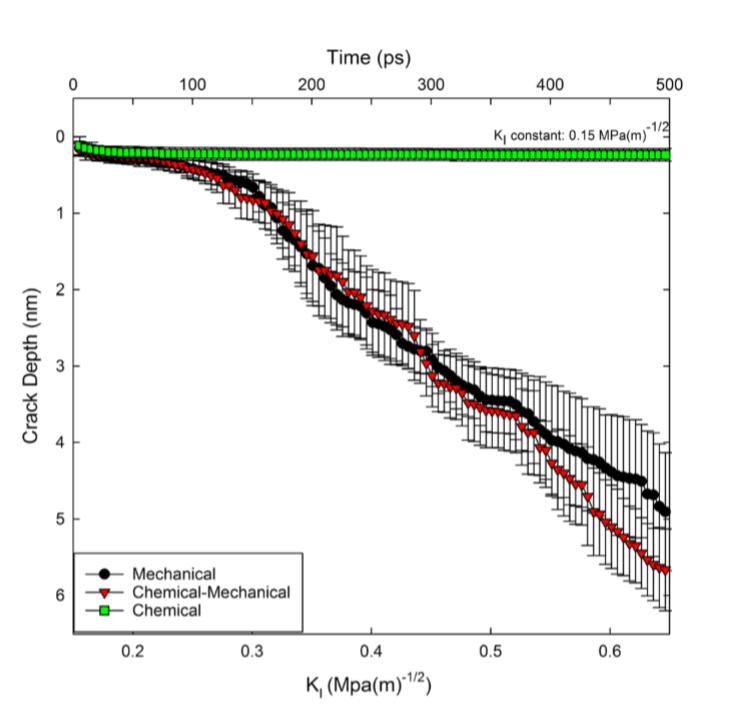
\includegraphics[width=11cm]{picture/crack_depth.PNG}
  \caption{Crack depth for silica systems under mechanical, chemical, and chemical-mechanical conditions.  Figure reproduced from~\protect\cite{chem_effects}}
  \label{crack_depth}
\end{figure}
\end{comment}

\begin{comment}
\begin{figure}[!b]
  \centering
  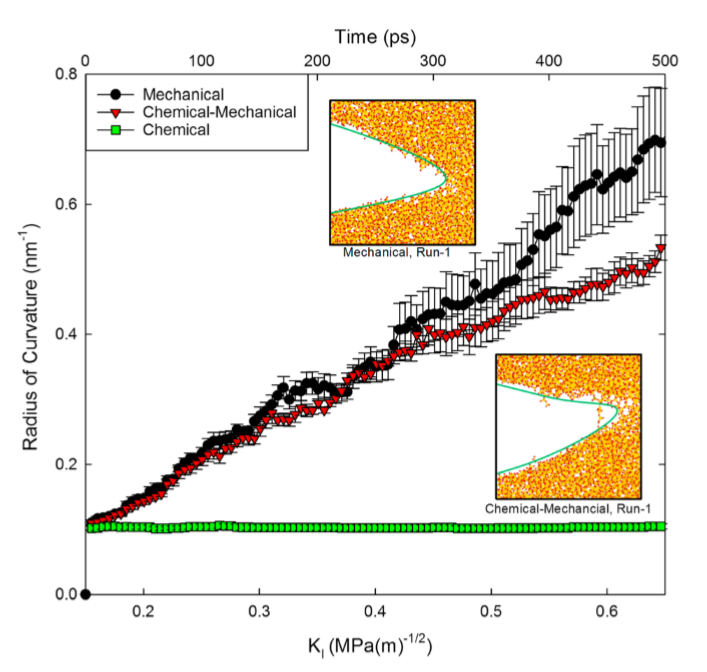
\includegraphics[width=11cm]{picture/crack_radius.PNG}
  \caption{Radius of curavture for silica systems under mechanical, chemical, and chemical-mechanical conditions. Figure reproduced from~\protect\cite{chem_effects}} 
  \label{crack_rad}
\end{figure}
\end{comment}



\begin{comment}
\begin{figure}[ht]
    \centering
    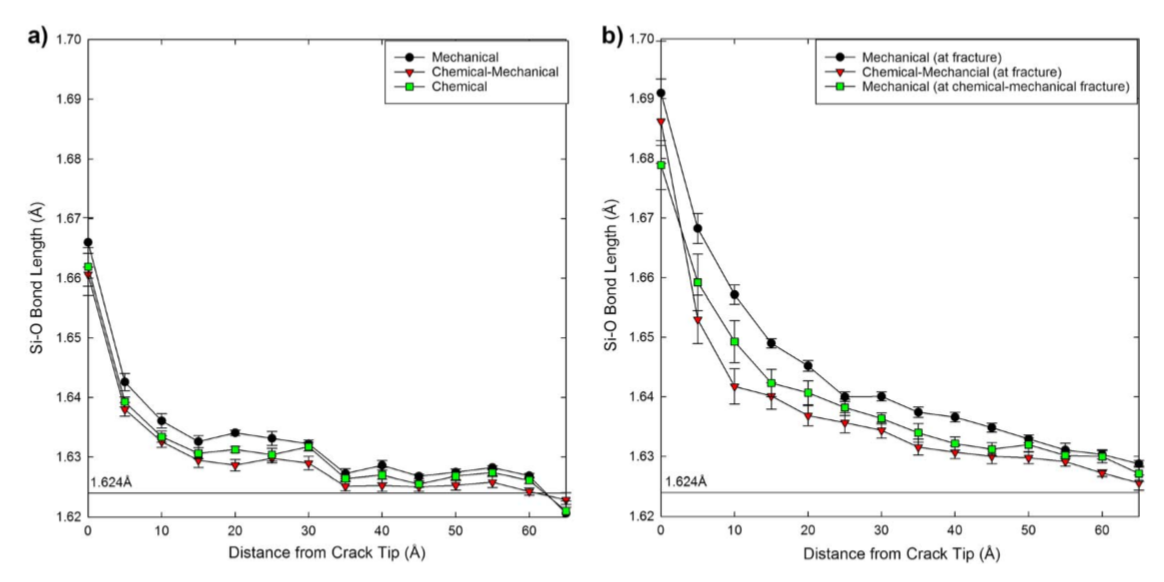
\includegraphics[width=10cm]{picture/AverageSiO.PNG}
    \caption{Average Si─O bond length based on distance from the crack tip at (a) initial conditions and (b) after loading.}
    \label{Average Si-O}
\end{figure}
\end{comment}


